
%(BEGIN_QUESTION)
% Copyright 2007, Tony R. Kuphaldt, released under the Creative Commons Attribution License (v 1.0)
% This means you may do almost anything with this work of mine, so long as you give me proper credit

In this process, two chemical streams are mixed together in a reactor vessel.  The ensuing chemical reaction is exothermic (heat-producing) and must be cooled by a water cooling system to prevent overheating of the vessel and piping.  A temperature transmitter (TT) senses the reaction product temperature and sends a 4-20 mA signal to a temperature indicating controller (TIC).  The controller then sends a 4-20 mA control signal to the temperature valve (TV) to throttle cooling water flow:

$$\includegraphics[width=15.5cm]{i02930x01.eps}$$

Suppose the temperature of the incoming cooling water suddenly increases.  That is, the cool water available to cool the exothermic process is not as cool as it used to be.  Describe in detail the effect this change in conditions will have on the performance of the cooling system.

\vskip 20pt \vbox{\hrule \hbox{\strut \vrule{} {\bf Suggestions for Socratic discussion} \vrule} \hrule}

\begin{itemize}
\item{} Is this process in danger of over- or under-heating from this change in cooling water temperature?
\item{} How hot do you think the cooling water can get before the control system simply fails to function?
\item{} If the control valve is signal-to-open, and the transmitter is direct-acting, does the controller need to be direct-acting or reverse-acting?
\end{itemize}


\underbar{file i02930}
%(END_QUESTION)





%(BEGIN_ANSWER)

%(END_ANSWER)





%(BEGIN_NOTES)

The controller should still be able to maintain the process temperature at setpoint, but it will have to open the cooling water valve further than usual to do so.

\vskip 10pt

Initially, the process temperature will spike up, and then it will correct with the temperature valve settling at a wider-open position than it was before.

%INDEX% Basics, control loop troubleshooting: determining effect of process load change
%INDEX% Process: exothermic chemical reactor (generic)

%(END_NOTES)


